\documentclass{article}\usepackage[]{graphicx}\usepackage[]{color}
%% maxwidth is the original width if it is less than linewidth
%% otherwise use linewidth (to make sure the graphics do not exceed the margin)
\makeatletter
\def\maxwidth{ %
  \ifdim\Gin@nat@width>\linewidth
    \linewidth
  \else
    \Gin@nat@width
  \fi
}
\makeatother

\definecolor{fgcolor}{rgb}{0.345, 0.345, 0.345}
\newcommand{\hlnum}[1]{\textcolor[rgb]{0.686,0.059,0.569}{#1}}%
\newcommand{\hlstr}[1]{\textcolor[rgb]{0.192,0.494,0.8}{#1}}%
\newcommand{\hlcom}[1]{\textcolor[rgb]{0.678,0.584,0.686}{\textit{#1}}}%
\newcommand{\hlopt}[1]{\textcolor[rgb]{0,0,0}{#1}}%
\newcommand{\hlstd}[1]{\textcolor[rgb]{0.345,0.345,0.345}{#1}}%
\newcommand{\hlkwa}[1]{\textcolor[rgb]{0.161,0.373,0.58}{\textbf{#1}}}%
\newcommand{\hlkwb}[1]{\textcolor[rgb]{0.69,0.353,0.396}{#1}}%
\newcommand{\hlkwc}[1]{\textcolor[rgb]{0.333,0.667,0.333}{#1}}%
\newcommand{\hlkwd}[1]{\textcolor[rgb]{0.737,0.353,0.396}{\textbf{#1}}}%

\usepackage{framed}
\makeatletter
\newenvironment{kframe}{%
 \def\at@end@of@kframe{}%
 \ifinner\ifhmode%
  \def\at@end@of@kframe{\end{minipage}}%
  \begin{minipage}{\columnwidth}%
 \fi\fi%
 \def\FrameCommand##1{\hskip\@totalleftmargin \hskip-\fboxsep
 \colorbox{shadecolor}{##1}\hskip-\fboxsep
     % There is no \\@totalrightmargin, so:
     \hskip-\linewidth \hskip-\@totalleftmargin \hskip\columnwidth}%
 \MakeFramed {\advance\hsize-\width
   \@totalleftmargin\z@ \linewidth\hsize
   \@setminipage}}%
 {\par\unskip\endMakeFramed%
 \at@end@of@kframe}
\makeatother

\definecolor{shadecolor}{rgb}{.97, .97, .97}
\definecolor{messagecolor}{rgb}{0, 0, 0}
\definecolor{warningcolor}{rgb}{1, 0, 1}
\definecolor{errorcolor}{rgb}{1, 0, 0}
\newenvironment{knitrout}{}{} % an empty environment to be redefined in TeX

\usepackage{alltt}
\usepackage[sc]{mathpazo}
\usepackage[T1]{fontenc}
\usepackage[utf8]{inputenc}
\usepackage{geometry}
\usepackage{amsmath} 
\usepackage{graphicx}
\usepackage{latexsym}
\geometry{verbose,tmargin=1.5cm,bmargin=2.5cm,lmargin=2.5cm,rmargin=2.5cm}
\setcounter{secnumdepth}{2}
\setcounter{tocdepth}{2}
\usepackage{url}
\usepackage[unicode=true,pdfusetitle,
 bookmarks=true,bookmarksnumbered=true,bookmarksopen=true,bookmarksopenlevel=2,
 breaklinks=false,pdfborder={0 0 1},backref=false,colorlinks=false]
 {hyperref}
\hypersetup{
 pdfstartview={XYZ null null 1}}
\IfFileExists{upquote.sty}{\usepackage{upquote}}{}
\begin{document}



\title{Introducci\'on a la Estad\'istica y Probabilidades CM-274}
\date{}
\maketitle

\vspace{0.3cm}

{\Large Variables Aleatorias}



\vspace{0.8cm}

Enlazar espacios muestrales y eventos a los datos, es proporcionado por el concepto de \textbf{Variables Aleatorias}.

\vspace{0.5cm}

Una \textbf{variable aleatoria} es una funci\'on $X:\Omega \rightarrow \mathbb{R}$ que asigna a un n\'umero real para cada resultado $\omega$.

\vspace{0.3cm}

\textbf{Ejemplo} Lanzamos una moneda $10$ veces. Sea $X(w)$ el n\'umero de caras en la secuencia $\omega$. Por ejemplo si $\omega = HHTHHTHHTT$, entonces $X(\omega) = 6$.

\vspace{0.3cm}

\textbf{Ejemplo} Lancemos dos monedas y sea $X$ el n\'umero de caras. Entonces, $\mathbb{P}(X = 0) = \mathbb{p}(\{TT\}) = 1/4$, $\mathbb{P}(X = 1) = \mathbb{P}(\{ HT, TH\}) = 1/2$ y $\mathbb{P}(X = 2) = \mathbb{P}(\{HH \} ) = 1/4$. Las variables aleatorias y su distribuci\'on puede ser resumida como sigue:

\vspace{0.5cm}

\begin{minipage}{2.5in}
%\begin{table}[h]
\centering
\begin{tabular}{l l |l}
$\omega$ & $\mathbb{P}(\{ \omega \})$ & $X(\omega)$\\
\hline
TT     & 1/4                        & 0         \\
TH     & 1/4                        & 1         \\
HT     & 1/4                        & 1         \\
HH     & 1/4                        & 2        
\end{tabular}
%\end{table} 
\end{minipage}
\begin{minipage}{2.5in}
%\begin{table}[h]
\centering
\begin{tabular}{l|l}
x & $\mathbb{P}(X = x)$ \\
\hline
0 & 1/4                 \\
1 & 1/2                 \\
2 &  1/4                  
\end{tabular}
%\end{table}
\end{minipage}

\vspace{0.5cm}


Dada una variable aleatoria $X$ y un subconjunto $A$ de la l\'inea real, definamos $X^{-}(A) = \{\omega \in \Omega: X(\omega) \in A \}$ y sea

\begin{align*}
\mathbb{P}(X \in A) = \mathbb{P}(X^{-1}(A)) = \mathbb{P}(\{\omega \in \Omega; X(\omega) \in A  \})\\
\mathbb{P}(X = x) = \mathbb{P}(X^{-1}(x)) = \mathbb{P}(\{\omega \in \Omega; X(\omega) = x  \}).
\end{align*}

\vspace{0.5cm}

\large{Funci\'on Distribuci\'on y Funci\'on de Probabilidad}

\vspace{0.3cm}

\textbf{Definici\'on} La \textit{Funci\'on Distribuci\'on  Acumulativa} o \texttt{CDF}, es la funci\'on $F_{X}: \mathbb{R} \rightarrow [0,1]$ es definido como

\begin{align}
F_{X}(x) = \mathbb{P}(X \leq x).
\end{align}

\vspace{0.5cm}

Los siguientes resultados muestran que la \texttt{CDF} completamente determina la \mbox{distribuci\'on} de una variable aleatoria.

\vspace{0.3cm}

\begin{enumerate}
\item Sea $X$ que tiene un \texttt{CDF} $F$ y sea $Y$ que tiene \texttt{CDF} $G$. Si $F(x) = G(x)$ para todo $x$, entonces $\mathbb{P}(X \in A) = \mathbb{P}(Y \in A)$ para todo $A$.
\item Una funci\'on $F: \mathbb{R} \rightarrow [0,1]$ es un \texttt{CDF} para alguna probabilidad $\mathbb{P}$ si y s\'olo si se cumplen las siguientes condiciones

\begin{enumerate}
\item $F$ es no decreciente: $x_1 < x_2$ implica $F(x_1) \leq F(x_2)$.
\item $F$ es normalizado: 
\[
\lim_{x \rightarrow -\infty}F(x) = 0
\]
y 

\[
\lim_{x \rightarrow \infty}F(x) = 1
\]
\item $F$ es continua por la derecha: $F(x) = F(x^{+})$ para todo $x$, donde
\[
F(x^{+}) = \lim_{y \rightarrow x}F(y) \qquad \mbox{si} \qquad y > x.
\]
\end{enumerate}
\end{enumerate}


\vspace{0.5cm}

\textbf{Ejemplo} Lanzamos una moneda dos veces y sea $X$ el n\'umero de caras. Entonces $\mathbb{P}(X = 0) = \mathbb{P}(X = 2) = 1/4$ y $\mathbb{P}(X = 1) = 1/2$. La funci\'on distribuci\'on es

\[
F_{X}(x) = \begin{cases}
0 & x < 0\\
1/4 & 0 \leq x < 1\\
3/4 & 1 \leq x < 2\\
1 & x \geq 2.
\end{cases}
\]

\vspace{0.2cm}

y el \texttt{CDF} es mostrado en la siguiente figura. Se debe notar que la funci\'on es continua por la derecha,no decreciente y es definida para todo $x$, incluso si la variable aleatoria toma los valores $0, 1$ y $2$.

\vspace{0.2cm}
\begin{figure}[h]
\centering
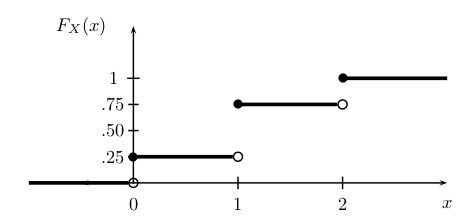
\includegraphics[scale=.55]{graff1-o.png}
%\caption{Modelo del problema}
\end{figure}

\vspace{0.5cm}

\textbf{Definici\'on} Si $X$ es discreta si toma valores contables $\{x_1, x_2, \dots \}$. Definimos la \textbf{\mbox{funci\'on} probabilidad} o \textbf{pmf} para $X$ por $f_{X}(x) = \mathbb{P}(X = x)$. 

\vspace{0.5cm}

As\'i, $f_{X}(x) \geq 0$ para todo $x \in \mathbb{R}$ y $\sum_{i}f_{X}(x_i) =1$. El \texttt{CDF} es relacionado a $f_{X}$ por

\[
F_{X}(x) = \mathbb{P}(X \leq x) = \sum_{x_i \leq x}f_{X}(x_i).
\]

\vspace{0.3cm}

La funci\'on probabilidad para el ejemplo  anterior es

\vspace{0.3cm}

\[
f_{X}(x) = \begin{cases}
1/ & x = 0\\
1/2 & x = 1\\
1/4 & x = 2\\
0 & \mbox{en otros casos}.
\end{cases}
\]

\vspace{0.2cm}

Como indica la siguiente figura

\vspace{0.2cm}

\vspace{0.2cm}
\begin{figure}[h]
\centering
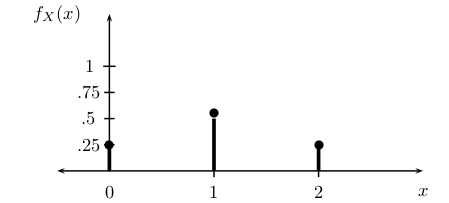
\includegraphics[scale=.55]{graff1-jk.png}
%\caption{Modelo del problema}
\end{figure}

\vspace{0.5cm}

\textbf{Definici\'on} Una variable aleatoria es \textbf{continua} si existe una funci\'on $f_X$ tal que $f_X(x) \geq 0$ para todo $x$, $\int_{-\infty}^{\infty}f_X(x)dx = 1$ y para todo $a \leq b$,

\begin{align}
\mathbb{P}(a < X < b) = \int_a^{b}f_{X}(x)dx.
\end{align}

La funci\'on $f_X$ es llamada \textbf{funci\'on densidad de probabilidad (PDF)}. Tenemos que

\[
F_{X}(x) = \int_{-\infty}^{x}f_{X}(t)dt
\]

y $f_{X}(x) = F_{X}^{'}(x)$ para todos los puntos $x$ donde $F_X$ es diferenciable.


\vspace{0.3cm}

\textbf{Ejemplo} Supongase que $X$ tiene \texttt{PDF}

\vspace{0.2cm}

\[
f_X(x) = \begin{cases}
1 & \mbox{para} \ \ 0 \leq x < 1 \\
0 & \mbox{en otros casos}
\end{cases}
\]


\vspace{0.2cm}

Claramente $f_{X} \geq 0$ y $\int f_X(x)dx = 1$. Una variable aleatoria con esta densidad se dice que tiene una distribuci\'on uniforme (\mbox{Uniform(0,1)}), lo que captura la idea, de escoger un punto entre 0 y 1.  El \texttt{CDF} est\'a dado por

\vspace{0.2cm}

\[
F_{X}(x) = \begin{cases}
0 & x < 0\\
x & 0 \leq x \leq 1\\
1 & x > 1.
\end{cases}
\]

y cuyo gr\'afico es 

\begin{figure}[h]
\centering
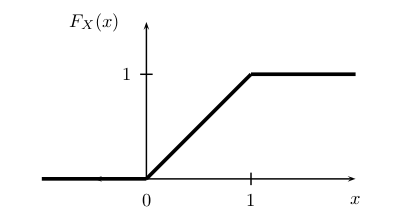
\includegraphics[scale=.55]{graff1-hg.png}
%\caption{Modelo del problema}
\end{figure}

\vspace{0.2cm}

\textbf{Ejemplo} Supongamos que $X$ tiene \texttt{PDF}

\[
f(x) = \begin{cases}
0 & \mbox{si} \  x < 0\\
\frac{1}{(1 + x)^2} & \mbox{en otros casos}.
\end{cases}
\]

\vspace{0.2cm}

Desde que $\int f(x)dx = 1$ esta es una bien definida \texttt{PDF}.

\vspace{0.3cm}


\textbf{Observaciones}

\vspace{0.2cm}

\begin{enumerate}
\item Si $X$ es continua, entonces $\mathbb{P}(X =x) = 0$ para cada $x$. 
\item No se debe pensar $f(x)$ como $\mathbb{P}(X=x)$. Esto se cumple, para variables aleatorias discretas.
\end{enumerate}

\vspace{0.3cm}

\textbf{Ejemplo} Sea 

\[
f(x) = \begin{cases}
0 & x < 0\\
\frac{1}{(1 + x)} & \mbox{ en otros casos.}
\end{cases}
\]

\vspace{0.2cm}

Esto no es un \texttt{PDF}, desde que $\int f(x)dx = \log \infty = \infty$.

\vspace{0.3cm}

\textbf{Teorema} Sea $F$ el \texttt{CDF} una variable aleatoria $X$. Entonces

\begin{enumerate}
\item $\mathbb{P}(X =x) = F(x) - F(x^{-}) $, donde $F(x^{-}) = \lim_{y \rightarrow x}F(y) \  \mbox{si} \  y < x \ \ (\lim_{y \uparrow x}F(y))$.
\item $\mathbb{P}(x < X \leq y = F(y) -F(x)$
\item $\mathbb{P}(X > x) = 1-F(x)$
\item Si $X$ es continua, entonces
\begin{align*}
F(b) -F(a) = \mathbb{P}(a < X < b) &= \mathbb{P}(a \leq X < b)\\
 = \mathbb{P}(a < X \leq b) &=  \mathbb{P}(a \leq X \leq b)
\end{align*}
\end{enumerate}

\vspace{0.3cm}

Definamos la inversa \texttt{CDF}, o \textbf{funci\'on cuantil}

\vspace{0.3cm}

\textbf{Definici\'on} Sea $X$ una variable aleatoria con \texttt{CDF} $F$. La \textit{inversa \texttt{CDF}} o \textit{funci\'on cuantil} es definida como

\[
F^{-1}(q) = \inf\{x: F(x) > q \}
\]
para $q \in [0,1]$. Si $F$ es estrictamente creciente y continua, entonces $F^{-1}(q)$ es el \'unico n\'umero real $x$ tal que $F(x) = q$.

\vspace{0.3cm}

Llamamos $F^{-1}(1/4)$ el \textit{el primer cuartil}, $F^{-}(1/2)$ la \textit{mediana} o \textit{segundo cuartil} y $F^{-1}(3/4)$, el tercer cuartil.

\vspace{0.3cm}

Dos variables aleatorias $X$ y $Y$ son \textbf{iguales en distribuci\'on} si $F_{X}(x) = F_{Y}(y)$ para todo $x$. Esto significa que las aseveraciones de probabilidad acerca de $X$ y $Y$ deben ser las mismas.


\newpage


{\Large Algunas importantes Variables Aleatorias Discretas}

\vspace{0.8cm}

\textbf{1.- Distribuci\'on Uniforme Discreta} Sea $k > 1$ un n\'umero entero. Supongamos que $X$ tiene \texttt{pmf} dado por

\[
f(x) = \begin{cases}
1/k & \mbox{para} \ 1, \dots ,k\\
0 & \mbox{ en otros casos.}
\end{cases}
\]

\vspace{0.2cm}

Decimos que $X$ tiene una distribuci\'on uniforme sobre $\{1, \dots, k \}$.

\vspace{0.5cm}

\textbf{2.-La Distribuci\'on de Bernoulli} Sea $X$ que representa una lanzamiento de una moneda. Entonces $\mathbb{P}(X = 1) = p$ y $\mathbb{P}(X= 0) = 1 - p$ para alg\'un $p \in [0,1]$, entonces decimos que $X$ tiene una distribuci\'on de Bernoulli, escrita como $X \sim\mbox{Bernoulli}$. La funci\'on \mbox{probabilidad} es $f(x) = p^{x}(1 - p)^{1-x}$ para $x \in \{0,1\}$.

\vspace{0.5cm}

\textbf{3.- Distribuci\'on Binomial} Supongamos que tenemos una moneda, que cae cara con una probabilidad $p$ para alg\'un $0 \leq p \leq 1$. Lanzamos la moneda $n$ veces y sea $X$ el n\'umero de caras. Asumimos que esos lanzamientos son independientes. Sea $f(x) = \mathbb{P}(X = x)$, el \texttt{pmf }. Se puede mostrar que


\[
f(x) = \begin{cases}
\binom{n}{x}p^{x}(1 - p)^{x} & \mbox{para} \ x =0, \dots ,n\\
0 & \mbox{ en otros casos.}
\end{cases}
\]

Una variable aleatoria con este \texttt{pmf} es llamada variable aleatoria Binomial y se puede escribir como $X \sim \mbox{Binomial}(n_1, p)$ y $X_2 \sim \mbox{Binomial}(n_2, p)$ entonces 

$X_1 + X_2 \sim \mbox{Binomial}(n_1 + n_2, p)$.


\vspace{0.5cm}

\textbf{4.- Distribuci\'on Geom\'etrica} $X$ tiene una distribuci\'on geom\'etrica con par\'ametro $p \in (0,1)$, escrito como $X \sim \mbox{Geom}(p)$, si

\[
\mathbb{P}(X = k) = p(1 -p)^{k -1}, \ \ k \geq 1.
\]

\vspace{0.2cm}

Tenemos a partir de esto que

\vspace{0.2cm}

\[
\sum_{k = 1}^{\infty}\mathbb{P}(X= k) = p\sum_{k = 1}^{\infty}(1 - p)^{k} = \frac{p}{ 1 - (1 - p)} = 1.
\]

\vspace{0.2cm}

Piensa en $X$ como el n\'umero de lanzamientos necesarios hasta  la primera cara, cuando una moneda es lanzada.

\vspace{0.5cm}

\textbf{5.-La Distribuci\'on de Poisson} $X$ tiene una distribuci\'on de Poisson con par\'ametro $\lambda$ escrita como $X \sim \mbox{Poisson} (\lambda)$ si

\[
f(x) = e^{-\lambda}\frac{\lambda^{x}}{x!} \ \ x \geq 0.
\]

\vspace{0.2cm}

Nota que

\[
\sum_{k = 0}^{\infty}f(x) = e^{-\lambda}\sum_{x = 0}^{\infty}\frac{\lambda^{x}}{x!} = e^{-\lambda}e^{\lambda} = 1. 
\]

\vspace{0.5cm}

La distribuci\'on de Poisson es usado a menudo como un modelo para eventos, como decaimiento radiactivo y accidentes de tr\'afico. Si $X_1\sim \mbox{Poisson}(\lambda_1)$ y  $X_2 \sim \mbox{Poisson}(\lambda_2)$ entonces $X_1 + X_2 \sim \mbox{Poisson}(\lambda_1 + \lambda_2)$.

\vspace{0.3cm}

Definimos las variables aleatorias como una aplicaci\'on de una espacio muestral $\Omega$ a $\mathbb{R}$ pero no mencionamos el espacio muestral en cualquiera de las distribuciones anteriores. El espacio muestral a menudo "desaparece", pero es realmente as\'i Vamos a construir un espacio de muestra expl\'icito de una variable aleatoria de Bernoulli. Sea $\Omega = [0,1]$ y definamos $\mathbb{P}$ saisfaciendo $\mathbf{P}([a, b]) = b -a$ para $0 \leq a \leq b \leq 1$. Fijemos $p \in [ 0,1]$ y definamos

\[
X(\omega) = \begin{cases}
1 & \omega \leq p\\
0 & \omega > p
\end{cases}
\]

\vspace{0.3cm}

Entonces $\mathbb{P}(X = 1) = \mathbb{P}(\omega \leq p) = \mathbf{P}([0, p]) = p$ y $\mathbb{P}(X = 0) = 1 -p$. As\'i $X \sim \mbox{Bernoulli}(p)$.


\vspace{0.8cm}


{\Large Algunas importantes Variables Aleatorias Continuas.}

\vspace{0.8cm}

\textbf{1.- La Distribuci\'on Uniforme} $X$ tiene una distribuci\'on Uniforme en (a,b), escrita como $X \sim \mbox{Uniform}(a,b)$ si

\[
f(x) = \begin{cases}
\frac{1}{b -a} & \mbox{para}\ x\in [a,b]\\
0 & \mbox{en otro caso}.
\end{cases}
\]
\vspace{0.2cm}

donde $a < b$. La funci\'on distribuci\'on es es

\[
F(x) = \begin{cases}
0 & x < a\\
\frac{x -a}{b -a} & x \in [a,b]\\
1 & x > b
\end{cases}
\]


\vspace{0.5cm}

\textbf{2.-Normal (Gaussiana)} $X$ tiene una distribuci\'on \textbf{Normal (Gaussiana)} con param\'etros $\mu$ y $\sigma$, denotado por $X \sim N(\mu, \sigma^2)$, si

\begin{align}
f(x) = \frac{1}{\sigma \sqrt{2\pi}}\exp\Bigl\{-\frac{1}{2\sigma^2}(x - \mu)^2 \Bigr\}, \ \ x \in \mathbb{R}
\end{align}

\vspace{0.3cm}

donde $\mu \in \mathbb{R}$ y $\sigma > 0$.  El par\'ametro $\mu$ es el "centro" (o media) de la distribuci\'on y $\sigma$ es la desviaci\'on est\'andar) de la distribuci\'on. La distribuci\'on normal juega un papel importante en probabilidad y estad\'istica pues muchos fen\'omenos en la naturaleza tienen distribuciones aproximadamente normales. Uno de los resultados m\'as importantes de la Estad\'istica el \textbf{Teorema del L\'imite Central} dice que la distribuci\'on de una suma de variables aleatorias puede aproximarse por una distribuci\'on normal, lo que hace a la distribuci\'on Gaussiana muy importante.

\vspace{0.3cm}

Decimos que $X$ tiene una \textbf{Distribuci\'on Normal Est\'andar} si $\mu = 0$ y $\sigma =1$, que se denota como $Z$. La $\texttt{PDF}$ y $\texttt{CDF}$ de una distribuci\'on normal es denotada por $\phi(z)$ y $\Phi(z)$. El $\texttt{PDF}$ de esta distribuci\'on es dibujado como


\vspace{0.2cm}
\begin{figure}[h]
\centering
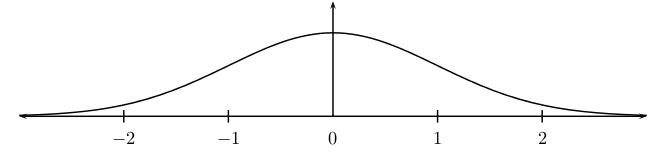
\includegraphics[scale=.55]{graff1-nm.png}
%\caption{Modelo del problema}
\end{figure}

\vspace{0.2cm}

Aqu\'i algunas propiedades

\begin{enumerate}
\item Si $X \sim N(\mu, \sigma^2)$, entonces $Z = (X - \mu)/\sigma \sim N(0,1)$.
\item Si $Z \sim N(0,1)$, entonces $X = \mu + \sigma Z \sim N(\mu, \sigma^2) $.
\item Si $X_i \sim N(\mu_i, \sigma_i^2), i=1,\dots,n$  son independientes, entonces

\[
\sum_{i = 1}^{n}X_i \sim N\Bigl(\sum_{i = 1}^{n}\mu_i, \sum_{i = 1}^{n}\sigma_i^2).
\]
\end{enumerate}
Se sigue desde $1.$ que si $X \sim N(\mu, \sigma^2)$ entonces

\begin{align*}
\mathbb{P}(a < X < b) = \mathbb{P}\Bigl( \frac{a - \mu}{\sigma} < Z < \frac{b - \mu}{\sigma}\Bigr)\\
= \Phi \Bigl( \frac{b - \mu}{\sigma} \Bigr) - \Phi \Bigl( \frac{a - \mu}{\sigma} \Bigr)
\end{align*}

\vspace{0.2cm}

As\'i podemos calcular las probabilidades, siempre que podamos obtener el \texttt{CDF} de una distribuci\'on normal est\'andar.


\vspace{0.5cm}


\textbf{Ejemplo} Supongamos que $X \sim N(3, 5)$. Encuentra $\mathbb{P}(X > 1)$. La soluci\'on es

\[
\mathbb{P}(X > 1) = 1 -\mathbb{P}(X < 1) = 1 -\mathbb{P}\Bigl(Z < \frac{1 -3}{\sqrt{5}}  \Bigr) = 1- \Phi(-0.8944) = 0.81.
\]

\vspace{0.3cm}

Ahora encontremos $q = \Phi^{-1}(0.2)$. Esto significa que tenemos que encontrar $q$ tal que $\mathbb{P}(X < q) = 0.2$. Podemos resolver esto, escribiendo

\[
0.2 = \mathbb{P}(X < q) = \mathbb{P}\Bigl(Z < \frac{q - \mu}{\sigma} \Bigr) = \Phi\Bigl(\frac{q - \mu}{\sigma} \Bigr).
\]

\vspace{0.2cm}

Desde la Tabla Normal, $\Phi(-0.8416) = 0.2$. Por tanto

\[
-0.8416 = \frac{q - \mu}{\sigma} = \frac{q - 3}{\sqrt{5}}
\]

y as\'i $q = 3  -0.8416\sqrt{5} = 1.1181.$


\vspace{0.5cm}

\textbf{3.-Distribuci\'on Exponencial} $X$ tiene una distribuci\'on Exponencial con per\'imetro $\beta$ y denotado por $X \sim \mbox{Exp}(\beta)$, si

\[
f(x) = \frac{1}{\beta}e^{-x/\beta}\ \ , x > 0
\]

\vspace{0.2cm}

donde $\beta > 0$. La distribuci\'on exponencial es usado para modelar el tiempo de vida de componentes electr\'onicos y el tiempo de espera entre ciertos eventos.

\vspace{0.5cm}

\textbf{4.- Distribuci\'on Gamma} Para $\alpha > 0$, la \textbf{Funci\'on Gamma} es definida como $\Gamma(\alpha) = \int_{0}^{\infty}y^{\alpha -1}e^{-y}dy$. $X$ tiene una distribuci\'on Gamma con par\'ametros $\alpha$ y $\beta$ denotado por $X \sim \mbox{Gamma}(\alpha, \beta)$, si

\[
f(x) = \frac{1}{\beta^{\alpha}\Gamma(\alpha)}x^{\alpha -1}e^{-x/\beta}\ \, x >0
\]

donde $\alpha, \beta > 0$. La distribuci\'on exponencial es s\'olo la distribuci\'on $\Gamma(1, \beta)$. Si $X_i \sim \mbox{Gamma}(\alpha_i, \beta)$ son independientes, entonces $\sum_{i = 1}^{n} X_i \sim \mbox{Gamma}(\sum_{i = 1}^{n} \alpha_i, \beta)$. 

\vspace{0.5cm}

\textbf{5.-Distribuci\'on Beta} $X$ tiene una distribuci\'on $\mbox{Beta}$ con par\'ametros $\alpha > 0$  y $\beta > 0$, denotado por $X \sim \mbox{Beta}(\alpha, \beta)$, si

\[
f(x) = \frac{\Gamma(\alpha + \beta)}{\Gamma(\alpha)\Gamma(\beta)}x^{\alpha -1}(1 -x)^{\beta -1}, \ \ 0< x < 1.
\]

\vspace{0.5cm}

\textbf{6.-Distribuci\'on t y de Cauchy} $X$ tiene una distribuci\'on $t$ con $\nu$ grados de libertad, escrito como $X \sim t_{\nu}$ si 

\[
f(x) = \frac{\Gamma(\frac{\nu +1}{2})}{\Gamma(\frac{\nu}{2})} = \frac{1}{(1 + \frac{x^2}{\nu})^{(\nu + 1)/2}}.
\]

\vspace{0.3cm}

\textbf{La distribuci\'on Cauchy} es un caso especial de la distribuci\'on $t$, correspondiendo a $\nu = 1$. La densidad es

\[
f(x) = \frac{1}{\pi(1 + x^2)}
\]

\vspace{0.2cm}

\begin{align*}
\int_{-\infty}^{\infty}f(x)dx = \frac{1}{\pi}\int_{-\infty}^{\infty}\frac{dx}{(1 + x^2)} =  \frac{1}{\pi}\int_{-\infty}^{\infty}\frac{d\tan^{-1}(x)}{dx}\\ =
\frac{1}{\pi}[\tan^{-1}(\infty) - \tan^{-1}(-\infty)] 
&=  \frac{1}{\pi}[\frac{\pi}{2} - (-\frac{\pi}{2})] = 1.
\end{align*}

\vspace{0.5cm}

\textbf{7.-La Distribuci\'on $\chi$} $X$ tiene una distribuci\'on $\chi^2$ con $p$ grados de libertad, que se escribe como $X \sim \chi_{p}^2$ si

\[
f(x) = \frac{1}{\Gamma(p/2)2^{p/2}}x^{(p/2)-1}e^{-x/2}, \ \ x >0.
\]

\vspace{0.3cm}

Si $Z_1, \dots, Z_p $ son variables aleatorias normales est\'andar independientes entonces $\sum_{i = 1}^{p}Z_i^{2} \sim \chi_{2}^{p}.$


\vspace{0.8cm}

{\Large Distribuciones Bivariadas}

\vspace{0.5cm}

Dado un par de variables aleatorias discretas $X$ y $Y$, se define el \texttt{jdf} \textit{(joint mass function)} por  $f(x,y) = \mathbb{P}(X =x, Y=y)$.

\vspace{0.3cm}


\textbf{Ejemplo} Aqu\'i una distribuci\'on bivariada para dos variables aleatorias $X$ y $Y$ tomando los valores $0$ o $1 $:

\vspace{0.3cm}


\begin{table}[h]
\centering
\begin{tabular}{l|ll|l}
      & Y = 0 & Y = 1 &     \\
      \hline
X = 0 & 1/9   & 2/9   & 1/3 \\
X = 1 & 2/9   & 4/9   & 2/3 \\
\hline
      & 1/3   & 2/3   &  1  
\end{tabular}
\end{table}

\vspace{0.2cm}

As\'i, $f(1,1) = \mathbb{P}(X = 1,y =1) = 4/9$.

\vspace{0.5cm}

\textbf{Definici\'on} En el caso continuo, llamamos a una funci\'on $f(x,y)$ un \texttt{PDF} para una variable aleatoria $(X,Y)$ si

\begin{enumerate}
\item $f(x,y) \geq 0$ para todo $(x,y)$.
\item $\int_{\infty}^{\infty}\int_{\infty}^{\infty}f(x,y)dxdy = 1$ y
\item Para alg\'un conjunto $A \subset \mathbb{R} \times \mathbb{R}, \mathbb{P}((X,Y) \in A) = \int \int_{A}f(x,y)dxdy$.
\end{enumerate}

\vspace{0.3cm}

\textbf{Ejemplo} Sea $(X,Y)$ que tiene densidad

\[
f(x,y)= \begin{cases}
cx^2y & \mbox{si}\ \  x^2 \leq y \leq 1\\
0 & \mbox{ en otro caso}.
\end{cases}
\]

\vspace{0.2cm}

Notemos primero que $-1 \leq x \leq 1$. Encontremos el valor de $c$. Fijemos un valor $x$ y dejemos que $y$ varie en su rango, el cu\'al es $x^2 \leq y \leq 1$.

\vspace{0.3cm}

As\'i

\begin{align*}
1 = \int\int f(x,y)dxdy = c\int_{-1}^{1}\int_{x^2}^{1}x^2ydydx \\
= c\int_{-1}^{1}x^2\Bigl[\int_{x^2}^{1}ydy\Bigr]dx = c \int_{-1}^{1}x^2\frac{1 -x^4}{2}dx = \frac{4c}{21}.
\end{align*}

\vspace{0.2cm}
\begin{figure}[h]
\centering
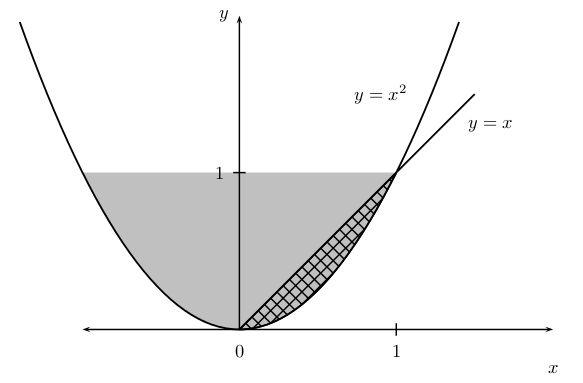
\includegraphics[scale=.45]{graff1-tu.png}
%\caption{Modelo del problema}
\end{figure}

\newpage

Ahora sea $c = 21/4$. Calculemos $\mathbb{P}(X \geq Y)$. Esto corresponde al conjunto $A = \{ (x,y); 0 \leq x \leq 1, x^2 \leq y \leq x\}$. (Se puede ver esto, en el diagrama de arriba). As\'i


\begin{align*}
\mathbb{P}(X \geq Y) = \frac{21}{4}\int_{0}^{1}\int_{x^2}^{x}x^2ydydx = \frac{21}{4}\int_{0}^{1}x^2\Bigl[\int_{x^2}^{x}ydy\Bigr]dx\\\ = \frac{21}{4}\int_{0}^{1}x^2\Bigl( \frac{x^2 - x^4}{2}\Bigr)dx = \frac{3}{20}.
\end{align*}


\vspace{0.8cm}

\textbf{Definici\'on} Si $(X,Y)$ tiene una distribuci\'on bivariada con $jdf$ $f_{X,Y}$, entonces el \texttt{mmf} \textit{marginal mass function para $X$} es definido por

\begin{align}
f_{X}(x) = \mathbb{P}(X=x) = \sum_{y}\mathbb{P}(X = x, Y=y) = \sum_{y}f(x,y)
\end{align}


\vspace{0.2cm}

y la \textit{marginal mass function para $Y$} es definido por

\begin{align}
f_{Y}(y) = \mathbb{P}(Y=y) = \sum_{x}\mathbb{P}(X = x, Y=y) = \sum_{x}f(x,y)
\end{align}


\vspace{0.3cm}

\textbf{Ejemplo} Supongamos que $f_{X,Y}$ es dado por la tabla siguiente. La distribuci\'on marginal para $X$  corresponde a las filas y la distribuci\'on marginal para $Y$ corresponde  a las \mbox{columnas}.


\vspace{0.3cm}

\begin{table}[h]
\centering
\begin{tabular}{l|ll|l}
      & Y = 0 & Y = 1 &     \\
      \hline
X = 0 & 1/10   & 2/10   & 3/10 \\
X = 1 & 3/10   & 4/10   & 7/10 \\
\hline
      & 4/10   & 6/10   &  1  
\end{tabular}
\end{table}

\vspace{0.2cm}

Por ejemplo, $f_{X}(0) = 3/10$ y $f_{X}(1) = 7/10$.


\vspace{0.8cm}

\textbf{Definici\'on} Para variables aleatorias continuas, las densidades marginales son

\vspace{0.2cm}

\begin{align}
f_{X}(x) = \int f(x,y)dy \ \ f_{Y}(y) = \int f(x,y)dx
\end{align}

\vspace{0.2cm}

Las correspondientes funciones de distribuci\'on marginal, son denotadas por $F_X$ y $F_{Y}$

\vspace{0.5cm}

\textbf{Ejemplo} Sea $(X,Y)$ tiene densidad
\[
f(x,y) = \begin{cases}
\frac{21}{4}x^2y & \mbox{si}\ x^2 \leq y \leq 1 \\
0 & \mbox{ en otros casos}.
\end{cases}
\]

\vspace{0.3cm}

As\'i

\vspace{0.2cm}


\[
f_{X}(x) = \int f(x,y)dy = \frac{21}{4}x^2\int_{x^2}^{1}ydy = \frac{21}{8}x^2(1 - x^4)
\]

\vspace{0.2cm}

para $-1 \leq x \leq 1$ y $f_{X}(x) = 0$ en otro caso.



\vspace{0.8cm}

\textbf{Definici\'on} Dos variables aleatorias $X$ y $Y$ son independientes, si para cada $A$ y $B$

\begin{align}
\mathbb{P}(X \in A, Y \in B) = \mathbb{P}(X \in A)\mathbb{P}(Y \in B)
\end{align}


\vspace{0.5cm}

\textbf{Teorema} Sean $X$ y $Y$ tienen un \texttt{PDF} $f_{X,Y}$. Entonces $X$ y $Y$ son independientes si y s\'olo si $f_{X,Y}(x,y) = f_{X}(x)f_{Y}(y)$ para todos los valores de $x$ y $y$.

\vspace{0.5cm}

\textbf{Ejemplo} Sean $X$ y $Y$ tienen la siguiente distribuci\'on

\vspace{0.3cm}

\begin{table}[h]
\centering
\begin{tabular}{l|ll|l}
      & Y = 0 & Y = 1 &     \\
      \hline
X = 0 & 1/4   & 1/4   & 1/2 \\
X = 1 & 1/4   & 1/4   & 1/2 \\
\hline
      & 1/2   & 1/2   &  1  
\end{tabular}
\end{table}

\vspace{0.2cm}

Entonces, $f_{X} (0) = f_{X}(1) = 1/2$ y $f_{Y}(0) = f_{Y}(1) = 1/2$. $X$ y $Y$ son independientes, ya que $f_{X}(0)f_{Y}(0) = f(0,0), f_{X}(0)f_{Y}(1) = f(0,1),  f_{X}(1)f_{Y}(0) = f(1,0), f_{X}(1)f_{Y}(1) = f(1,1)$. Pero si $X$ y $Y$ tienen la misma distribuci\'on

\vspace{0.2cm}

\begin{table}[h]
\centering
\begin{tabular}{l|ll|l}
      & Y = 0 & Y = 1 &     \\
      \hline
X = 0 & 1/2   & 0    & 1/2 \\
X = 1 & 0     & 1/2   & 1/2 \\
\hline
      & 1/2   & 1/2   &  1  
\end{tabular}
\end{table}

\vspace{0.3cm}

ellas no son independientes, ya que $f_{X}(0)f_{Y}(1) = (1/2)(1/2) = 1/4$, pero $f(0,1) = 0$.

\vspace{0.3cm}

\textbf{Ejemplo} Supongamos que $X$ y $Y$ son indepedientes y tienen la misma densidad

\[
f(x) = \begin{cases}
2x & \mbox{si}\  \ 0 \leq x \leq 1\\
0  & \mbox{en otros casos}
\end{cases}
\]

\vspace{0.2cm}

Encontremos $\mathbb{P}(X + Y \leq 1)$. Usando independencia, tenemos que  la \texttt{jdf} es

\[
f(x,y) = f_{X}(x)f_{Y}(y) = \begin{cases}
4xy & \mbox{si}\ \  0 \leq x \leq 1,\ \ 0 \leq y \leq 1\\
0 & \mbox{en otros casos}.
\end{cases}
\]

\vspace{0.5cm}

Ahora,

\vspace{0.3cm}

\begin{align*}
\mathbb{P}(X +  Y \leq 1) &= \int \int_{x + y \leq 1}f(x,y)dydx \\
&= 4\int_{0}^{1}x\Bigl[\int_{0}^{1-x}ydy \Bigr]dx \\
&=4 \int_{0}^{1}x\frac{(1 - x)^2}{2}dx = \frac{1}{6}.
\end{align*}

\vspace{0.3cm}

\textbf{Teorema}  Supongamos que el rango de $X$ y $Y$ es un rect\'angulo (posiblemente infinito). Si $f(x,y) = g(x)h(y)$ para alg\'un $g$ y $h$ (no necesariamente funciones de densidad) entonces $X$ y $Y$ son independientes.

\vspace{0.3cm}

\textbf{Ejemplo} Sean $X$ y $Y$ con densidad

\[
f(x,y) =\begin{cases}
2e^{-(x + 2y)} & \mbox{si} \ \ x > 0 \ \ y \ \ y > 0\\
0 & \mbox{en otros casos}.
\end{cases}
\]

\vspace{0.3cm}

El rango de $X$ y $Y$ es el rect\'angulo $(0, \infty) \times (0, \infty)$. Podemos escribir $f(x, y) = g(x)h(y)$, donde $g(x) = 2e^{-x}$ y $h(y) = e^{-2y}$. As\'i, $X$ y $Y$ son independientes.

\vspace{0.8cm}


Si $X$ y $Y$ son discretas, entonces podemos calcular la distribuci\'on condicional de $X$ dado que hemos observado $Y = y$. Especificamente, $\mathbb{P}(X =x| Y=y) = \mathbb{P}(X = x,Y=y)/\mathbb{P}(Y=y)$. Esto conduce a la definici\'on \texttt{cpmf} o \textit{Conditional probability mass function}.

\vspace{0.4cm}

\textbf{Definici\'on} La \texttt{cpmf} es

\[
f_{X|Y}(x|y) = \mathbb{P}(X = x| Y=y) = \frac{\mathbb{P}(X = x, Y=y)}{\mathbb{P}(Y = y)} = \frac{f_{X,Y}(x,y)}{f_{Y}(y)}
\]

\vspace{0.2cm}

si $f_{Y} > 0$.

\vspace{0.2cm}

\textbf{Definici\'on} Para variables aleatorias continuas, la \texttt{cpdf}, \textit{Conditional probability density function} es

\[
f_{X|Y}(x|y) = \frac{f_{X|Y}(x,y)}{f_{Y}(y)}
\]

\vspace{0.3cm}

asumiendo que $f_{Y}(y) > 0$. Entonces,

\[
\mathbb{P}(X \in A| Y=y) = \int_{A}f_{X|Y}(x|y)dx.
\]

\vspace{0.5cm}

\textbf{Ejemplo} Sean $X$ y $Y$, que tienen una distribuci\'on uniforme sobre un cuadrado unidad. As\'i $f_{X|Y}(x|y) = 1$, para $0 \leq x \leq 1$ y $0$ en otros casos. Dado $Y =y$, $X$ es $\mbox{Uniform}(0.1)$. Podemos escribir esto como $X|Y = y \sim \mbox{Uniform}(0,1)$.

\vspace{0.5cm}

\textbf{Ejemplo} Supongamos que $X \sim \mbox{Uniform}(0,1)$. Despu\'es de obtener un valor de $X$, generamos $Y|X = x \sim \mbox{Uniform}(x,1)$. La distribuci\'on marginal de $Y$ se puede calcular a partir de

\[
f_{X}(x) = \begin{cases}
1 & \mbox{si}\ \ 0 \leq x \leq 1\\
0 & \mbox{ en otros casos}.
\end{cases}
\]

y 

\[
f_{Y|X}(y|x) = \begin{cases}
\frac{1}{1 -x}& \mbox{si}\ \ 0 < x < y < 1 \\
0 & \mbox{en otros casos}.
\end{cases}
\]

\vspace{0.3cm}

As\'i

\[
f_{X,Y}(x,y) = f_{Y|X}(y|x)f_{X}(x) = \begin{cases}
\frac{1}{1 -x}& \mbox{si}\ \ 0 < x < y < 1 \\
0 & \mbox{en otros casos}.
\end{cases}
\]

\vspace{0.3cm}

La distribuci\'on marginal para $Y$ es

\[
f_{Y}(y) = \int_{0}^{y}f_{X,Y}(x,y)dx = \int_{0}^{y}\frac{dx}{1 -x} = -\int_{1}^{1- y}\frac{du}{u} = -\log(1-y)
\]

\vspace{0.3cm}

para $0 < y < 1$.

\vspace{0.8cm}

{\Large Distribuciones Multivariadas y Muestras Id\'enticamente Distribuidas e Independientes}

\vspace{0.5cm}

Sea $X = (X_1,\dots, X_n)$ donde $X_1, \dots, X_n$ son variables aleatorias. Llamamos a $X$ \textbf{Vector Aleatorio}. $f(x_1,\dots,x_n)$ denota el \texttt{PDF}. Es posible definir los mismos conceptos, de la misma manera que las distribuciones multivariadas. Decimos que $X_1,\dots, X_n$ son independientes si, para cada $A_1, \dots, A_n$

\begin{align}
\mathbb{P}(X_1 \in A_1,  \dots, X_n \in A_n) = \prod_{i=1}^{n}\mathbb{P}(X_i \in A_i).
\end{align}

\vspace{0.3cm}

Es suficiente verificar que $f(x_1,\dots, x_n) = \prod_{i = 1}^{n}f_{X_{i}}(x_i) $.


\vspace{0.5cm}

\textbf{Definici\'on} Si $X_1,\dots X_n$ son independientes y cada uno de ellos tiene la misma distribuci\'on marginal con \texttt{CDF} $F$, decimos que $X_1, \dots, X_n$ son id\'enticamente distribuidas e independientes y escribimos como

\vspace{0.3cm}

\[
X_1, \dots, X_n \sim F
\]

\vspace{0.3cm}

Si $F$ tiene densidad $f$, escribimos tambi\'en $X_1, \dots, X_n \sim f$. Llamamos a $X_1, \dots, X_n$ una muestra aleatoria de tama\~no $n$ desde $F$.


\vspace{0.8cm}


{\Large Dos Importantes Distribuciones Multivariadas}

\vspace{0.5cm}

\textbf{Multinomial} La versi\'on multivariada de la Binomial, es llamada \texttt{multinomial}. Considere la posibilidad de extraer una bola de una urna que tiene bolas con $k$ colores, etiquetados como \texttt{'color 1', 'color 2', \dots 'color k'}. Sea $p = (p1, \dots, p_k)$ donde $p_j \geq 0$ y $\sum_{j = 1}^{k}p_j = 1$ y supongamos que $p_j$ es la probabilidad de encontrar una bola de color $j$. Lanzamos $n$ veces (independientes lanzamientos con reemplazamiento) y sea $X = (X_1, \dots, X_k)$ donde $X_j$ es el n\'umero de veces que el color $j$ aparece. Por lo tanto $n = \sum_{j= 1}^{k}X_j$, as\'i decimos que $X$ tiene una distribuci\'on Multinomial $\mbox{Multinomial}(n,p)$. La funci\'on probabilidad es

\begin{align}
f(x) = \binom{n}{x_1\dots x_k}p_{1}^{x_1}\cdots p_{k}^{x_k}
\end{align}

\vspace{0.2cm}

donde 

\vspace{0.2cm}

\begin{align*}
\binom{n}{x_1\dots x_k} = \frac{n!}{x_1!\cdots x_k!}.
\end{align*}

\vspace{0.2cm}

\textbf{Propiedad} Supongamos que $X \sim \mbox{Multinomial(n, p)}$, donde $X = (X_1,\dots, X_k$ y $p = (p_1, \dots, p_k)$. La distribuci\'on marginal de $X_j$ es $\mbox{Binomial}(n, p_j)$.


\vspace{0.5cm}

\textbf{Normal Multivariada} La distribuci\'on normal univariada tiene dos par\'ametros  $\mu$ y $\sigma$. En la versi\'on multivariada, $\mu$ es un vector y $\sigma$ es reemplazada por una matriz $\Sigma$. Para empezar

\[
Z = \begin{pmatrix}
Z_1 \\
\vdots\\
Z_k
\end{pmatrix}
\]

\vspace{0.3cm}

donde $Z_1, \dots, Z_k \sim N(0,1)$ son independientes. La densidad de $Z$ es

\begin{align*}
f(z) = \prod_{i = 1}^{k}f(z_i) = \frac{1}{(2\pi)^{k/2}}\exp\Bigl\{-\frac{1}{2}\sum_{j = 1}^{k}z_j^{2}\Bigr\}\\
= \frac{1}{(2\pi)^{k/2}}\exp\Bigl\{-\frac{1}{2}z^{T}z\Bigr\}.
\end{align*}

\vspace{0.3cm}

Decimos que $Z$ tiene una distribuci\'on multivariada est\'andar escrita como $Z \sim N(0,I)$, donde $0$ representa el vector de $K$ ceros y $I$ es la matriz identidad  de orden $k \times k$. De manera m\'as general, un vector $X$ tiene una distribuci\'on Normal Multivariada, denotada por $X \sim N(\mu, \Sigma)$, si tiene una densidad

\vspace{0.3cm}

\begin{align}
f(x; \mu, \Sigma) = \frac{1}{(2\pi)^{k/2}\vert (\Sigma)\vert^{1/2}}\exp \Bigl\{-\frac{1}{2}(x - \mu)^{T}\Sigma^{-1}(x - \mu) \Bigr\}
\end{align}

\vspace{0.3cm}


donde $\vert \Sigma \vert$, denota el determinante de $\Sigma$, $\mu$ es un vector de longitud $k$ y $\Sigma$ es una matriz sim\'etrica, definida positiva. Colocando $\mu = 0$ y $\Sigma = I$ tenemos la distribuci\'on Normal Est\'andar.

\vspace{0.3cm}

desde que  $\vert \Sigma \vert$ es sim\'etrica y definida positiva, existe una matriz $\Sigma^{1/2}$ llamada la ra\'iz cuadrada de $\Sigma$ con las siguientes propiedades: 

\begin{enumerate}
\item  La matriz $\Sigma^{1/2}$ es sim\'etrica.
\item $\Sigma = \Sigma^{1/2}\Sigma^{1/2}$.
\item $\Sigma^{1/2}\Sigma^{-1/2} = \Sigma^{-1/2}\Sigma^{1/2} = I$ donde $\Sigma^{-1/2} = (\Sigma^{1/2})^{-1}$
\end{enumerate}

\vspace{0.5cm}

\textbf{Teorema} Si $Z \sim N(0,I)$ y $X = \mu + \Sigma^{1/2}Z$ entonces $X \sim N(\mu, \Sigma)$. De otro lado, si $X \sim N(\mu, \Sigma)$ entonces $\Sigma^{-1/2}(X -\mu) \sim N(0,I)$.


\vspace{0.5cm}

Supongamos que particionamos un vector Normal aleatorio $X$, como $X = (X_a, X_b)$. De manera similar tenemos la partici\'on $\mu = (\mu_a, \mu_b)$ y

\vspace{0.3cm}


\[
\Sigma = \begin{pmatrix}
\Sigma_{aa} & \Sigma_{ab} \\
\Sigma_{ba} & \Sigma_{bb}
\end{pmatrix}
\]


\vspace{0.5cm}

\textbf{Teorema} Sea $X \sim N(\mu, \Sigma)$. Entonces

\begin{enumerate}
\item La distribuci\'on marginal de $X_a$ es $X_a \sim N(\mu_a, \Sigma_{aa})$.
\item La distribuci\'on condicional de $X_b$ dado $X_a = x_a$ es

\[
X_b|X_a = x_a \sim N(\mu_b + \Sigma_{ba}\Sigma_{aa}^{-1}(x_a - \mu_a), \Sigma_{bb} -\Sigma_{ba}\Sigma_{aa}^{-1}\Sigma_{ab}).
\]
\item Si $a$ es un vector entonces $a^{T}X \sim N(a^{T}\mu, a^{T}\sum a)$.
\item $V = (X -\mu)^{T}\Sigma^{-1}(X - \mu) \sim \chi_{k}^{2}$.
\end{enumerate}

\vspace{0.8cm}


{\Large  Transformaci\'on de  Variables Aleatorias}

\vspace{0.5cm}

Supongamos que $X$ es una variable aleatoria con \texttt{PDF} $f_X$ y \texttt{CDF} $F_X$ . Sea $Y = r(X)$ una funci\'on de $X$, llamada una \textbf{transformaci\'on de X}. Calcular el  \texttt{PDF}  y \texttt{CDF} de $Y$ en el caso discreto, por ejemplo tenemos

\begin{align*}
f_{Y}(y) &= \mathbb{P}(Y=y) = \mathbb{P}(r(X) =y)\\
& = \mathbb{P}(\{x; r(x) = y\}) = \mathbb{P}(X \in r^{-1}(y))
\end{align*}

\vspace{0.3cm}

\textbf{Ejemplo} Sea $\mathbb{P}(X = -1) = \mathbb{P}(X = 1) = 1/4$ y $\mathbb{P}(X = 0) = 1/2$. Sea $Y = X^2$. Entonces, $\mathbb{P}(Y = 0) = \mathbb{P}(X = 0) = 1/2$ y $\mathbb{P}(Y = 1) = \mathbb{P}(X = 1) + \mathbb{P}(X = -1) = 1/2$. Resumiendo


\vspace{0.5cm}



\begin{minipage}{2.5in}
%\begin{table}[h]
\centering
\begin{tabular}{l l }
$x$ & $f_{X}(x)$ \\
\hline
-1     & 1/4   \\                     
0     & 1/2   \\                
1     & 1/4                        
\end{tabular}
%\end{table} 
\end{minipage}
\begin{minipage}{2.5in}
%\begin{table}[h]
\centering
\begin{tabular}{l l}
y & $f_Y(y)$ \\
\hline
0 & 1/2                 \\
1 & 1/2                 
\end{tabular}
%\end{table}
\end{minipage}

\vspace{0.5cm}


El caso es continuo, es m\'as dificil. Aqu\'i tres pasos para encontrar $f_Y$:

\vspace{0.3cm}

\begin{enumerate}
\item Para cada $y$, encuentra el conjunto $A_y =  \{x: r(x) \leq y \}$.
\item Encontrar el \texttt{CDF}

\begin{align*}
F_{Y}(y) = \mathbb{P}(Y \leq y) = \mathbb{P}(r(X) \leq y)\\
   = \mathbb{P}(\{x : r(x) \leq y \})\\
   = \int_{A_y}f_{X}(x)dx 
\end{align*}
\item El \texttt{PDF} es $f_{Y}(y) = F_{Y}^{'}(y)$.
\end{enumerate}


\vspace{0.5cm}

\textbf{Ejemplo} Sea $f_{X}(x) = e^{-x}$ para $x > 0$. As\'i, $F_{X}(x) = \int_{0}^{x}f_{X}(s)ds = 1 -e^{-x}$. Sea $Y = r(X) = \log(X)$. Entonces $A_y = \{x: x\leq e^{y} \}$ y

\begin{align*}
F_{Y}(y) = &\mathbb{P}(Y\leq y) = \mathbb{P}(\log X \leq Y)\\
= & \mathbb{P}(X \leq e^y) = F_{X}(e^y) =  1- e^{-e^{y}}.
\end{align*}

\vspace{0.3cm}

Por tanto, $f_{Y}(y) = e^ye^{-e^{y}}$ para $y \in \mathbb{R}$.


\vspace{0.5cm}

Si tenemos por ejemplo, $X$ y $Y$ variables aleatorias, veamos como conocer la distribuci\'on de $X/Y, X +Y, \max\{X,Y \} $ o $\min\{X,Y \}$. Sea $Z = r(X,Y)$, los pasos para encontrar $f_{Z}$ son los mismo de antes

\begin{enumerate}
\item Para cada $z$, encuentra el conjunto $A_z =  \{(x,y): r(x,y) \leq z \}$.
\item Encontrar el \texttt{CDF}

\begin{align*}
F_{Z}(z) = \mathbb{P}(Z \leq z) = \mathbb{P}(r(X,Y) \leq z)\\
   = \mathbb{P}(\{(x,y) : r(x,y) \leq z \})\\
   = \int \int_{A_z}f_{X,Y}(x,y)dxdy 
\end{align*}
\item El \texttt{PDF} es $f_{Z}(z) = F_{Z}^{'}(z)$.
\end{enumerate}

\vspace{0.3cm}

\textbf{Ejemplo} Sea $X_1, X_2 \sim \mbox{Uniform}(0.1)$ independientes. Encontremos la densidad de $Y = X_1 + X_2$ en efecto la  \texttt{jdf} de $(X_1,X_2)$ es

\vspace{0.2cm}

\[
f(x_1, x_2) = \begin{cases}
1 & 0< x_1 < 1, 0 < x_2 < 1\\
0 & \mbox{en otros casos}
\end{cases}
\]


\vspace{0.3cm}

Sea $r(x_1, x_2) = x_1 + x_2$. Ahora

\vspace{0.3cm}

\begin{align*}
F_{Y}(y) &= \mathbb{P}(Y \leq y)= \mathbb{P}(r(X_1,X_2) \leq y)\\
& = \mathbb{P}( \{(x_1, x_2): r(x_1, x_2)\leq y \}) = \int \int_{A_y}f(x_1, x_2)dx_1dx_2.
\end{align*}

\vspace{0.2cm}

Para encontrar $A_y$, suponemos primero que $0 < y \leq 1$. Entonces $A_y$ es el tri\'angulo con v\'ertices $(0,0), (y,0)$ y $(0.y)$.. En este caso $\int \int_{A_y}f(x_1, x_2)dx_1dx_2$ es el \'area del tri\'angulo, es decir $y^2/2$. Si $1 < y < 2$, entonces $A_y$ es todo el cuadrado unitario, menos el tri\'angulo con v\'ertices $(1, y-1),(1,1), (y -1,1)$. Este conjunto tiene \'area $1 - (2 -y)^2/2$ 

\vspace{0.2cm}

\begin{figure}[h]
\centering
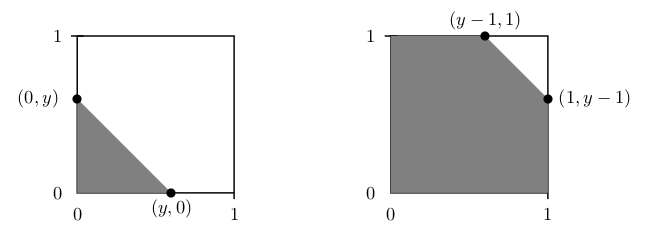
\includegraphics[scale=.65]{graff1-vw.png}
%\caption{Modelo del problema}
\end{figure}

\vspace{0.2cm}

Por tanto

\vspace{0.2cm}

\[
F_{Y}(y) = \begin{cases}
0 & y < 0\\
\frac{y^2}{2} & 0 \leq y < 1 \\
1 -\frac{(2 -y)^2}{2} & 1 \leq y < 2\\
1 & y \geq 2
\end{cases}
\]

\vspace{0.2cm}

Por diferenciaci\'on el \texttt{PDF} es

\[
f_{Y}(y)=\begin{cases}
y & 0 \leq y \leq 1 \\
2 -y & 1\leq y \leq 2\\
0 & \mbox{ en otros casos}.
\end{cases}
\]
 \end{document}
